\chapter{Certificate Server}
A \CS manages its own AD certificate issued by \ISDC and the
certificates of all entities within an \AD, and handles certificate
requests. In addition, a \ISDC certificate server manages the \RT file
on which all entities within an \ISD establish {trust}. A \CS contains
a key server, which generates and distributes keys for securing
internal (i.e., intra-AD) communication.

\section{Root of Trust File} \label{subsec:root-of-trust}
The \RT file contains the list of all \ISDC members and their
signatures. The file keeps track of the current policy number and the
\ADs that signed the policy. The policy is used as a {\bf \em root of
trust} by which all \ADs in the ISD establish their trust. The notion
of root of trust is crucial in the SCION architecture due to the
hierarchical structure of the \ISD. As a consequence, the ISD
membership is strictly limited and agreed by the current members.
This is enforced by restricting the update privilege of the \PF. More
specifically, the current members of \ISDC define the minimum number
of \ADs that should provide their signature for updating the \RT file
-- defined as {\em Policy Quorum Threshold} ($P_{th}$). Furthermore,
the \ISDC members define the minimum number of \AD signatures to grant
a new \AD's joining to the \ISDC and to issue a certificate for the
AD. This number, defined as {\em Certificate Quorum Threshold}
($C_{th}$), is also included in the \PF. Hence, an \AD, if it is
approved to join a \ISDC, would be included in the \RT file that is
signed by at least $C_{th}$ \ISDC \ADs. Figure~\ref{fig:rot-file}
shows the contents of the \RT file constructed in the XML format.

\begin{SaveVerbatim}{RotSection}
<ROT>
	<header> 
	<!-- Why we just switch this header field to ROT header properties -->
		<policyNumber>"policyNumber"</policyNumber>
		<ISDID>"Isolation Domain ID"</ISDID>
		<policyThreshold>"policyThreshold"</policyThreshold>
		<certificateThreshold>"certificateThreshold"</certificateThreshold>
	</header>
	<coreADs>
		<coreAD>
			<AID>"AID"</AID>
			<publicKey>"publicKey"</publicKey>
		</coreAD>
		...
	</coreADs>
	<signatures>
		<coreAD>
			<AID>"AID"</AID>
			<sign>"Signature"</sign>
		</coreAD>
		...
	</signatures>
</ROT>
\end{SaveVerbatim}

\begin{figure}[h]
\centering
%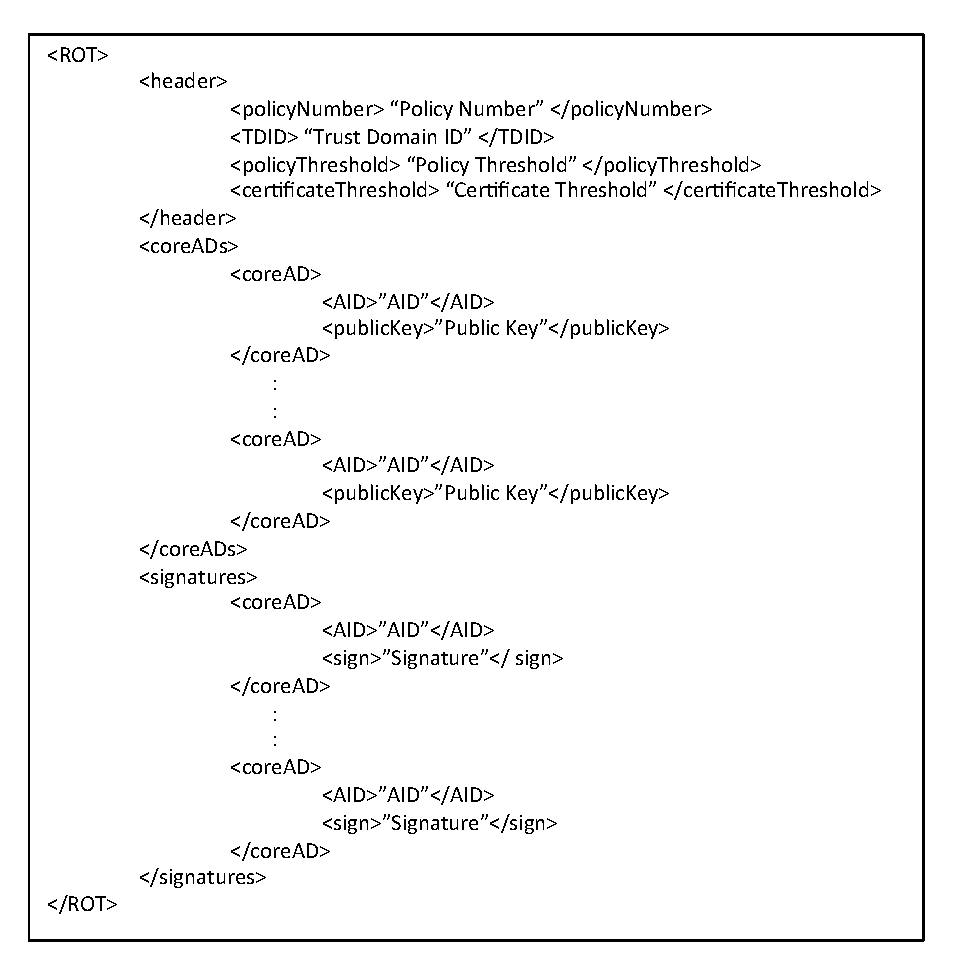
\includegraphics[width=.7\columnwidth]{./fig/rotfile.eps}
%\caption{\RT File Format}\label{fig:rot-file}
\begin{center}
	\fbox{
		\begin{minipage}{\columnwidth}
			\BUseVerbatim[fontsize=\footnotesize]{RotSection}
		\end{minipage}
	}
\end{center}
\caption{\RT File Format}\label{fig:rot-file}
\end{figure}

\tenma{We can define DTD (Document Type Definition) for XML structure.}

\paragraph{Header}
The header contains the \ISDC policy information listed below. 

\begin{enumerate}
\item Isolation Domain ID (ISD ID or TID) : Globally unique Isolation Domain identifier.
\item Policy ID : Current version number of \PF.
\item Policy Quorum Threshold : Minimum number of \ISDC \ADs needed to generate a new \RT file. 
\item Certificate Quorum Threshold : Minimum number of \ISDC \ADs needed to issue a new certificate for an \AD.
\end{enumerate}
\tenma{Should we keep a timestamp field or identifier to distinguish the difference of versions?}

\paragraph{\ISDC member list}
The \ISDC member list contains the information of all \ISDC members. Each \AD has the following elements:
\begin{enumerate}
\item \AD ID (AID).
\item \AD's public key.
\end{enumerate}

\paragraph{Signatures}
The signatures element contains the signatures of the \ISDC ADs that signed the current \RT file.
\begin{enumerate}
\item AD ID (AID).
\item \AD's signature computed over the header and the \ISDC member list.
\end{enumerate}

\tenma{Updating RoT files is also needed to included since certificate would be expired or revoked
in some conditiona.}

\section{Certificate Management} 

\begin{figure*}[ht]
\centering
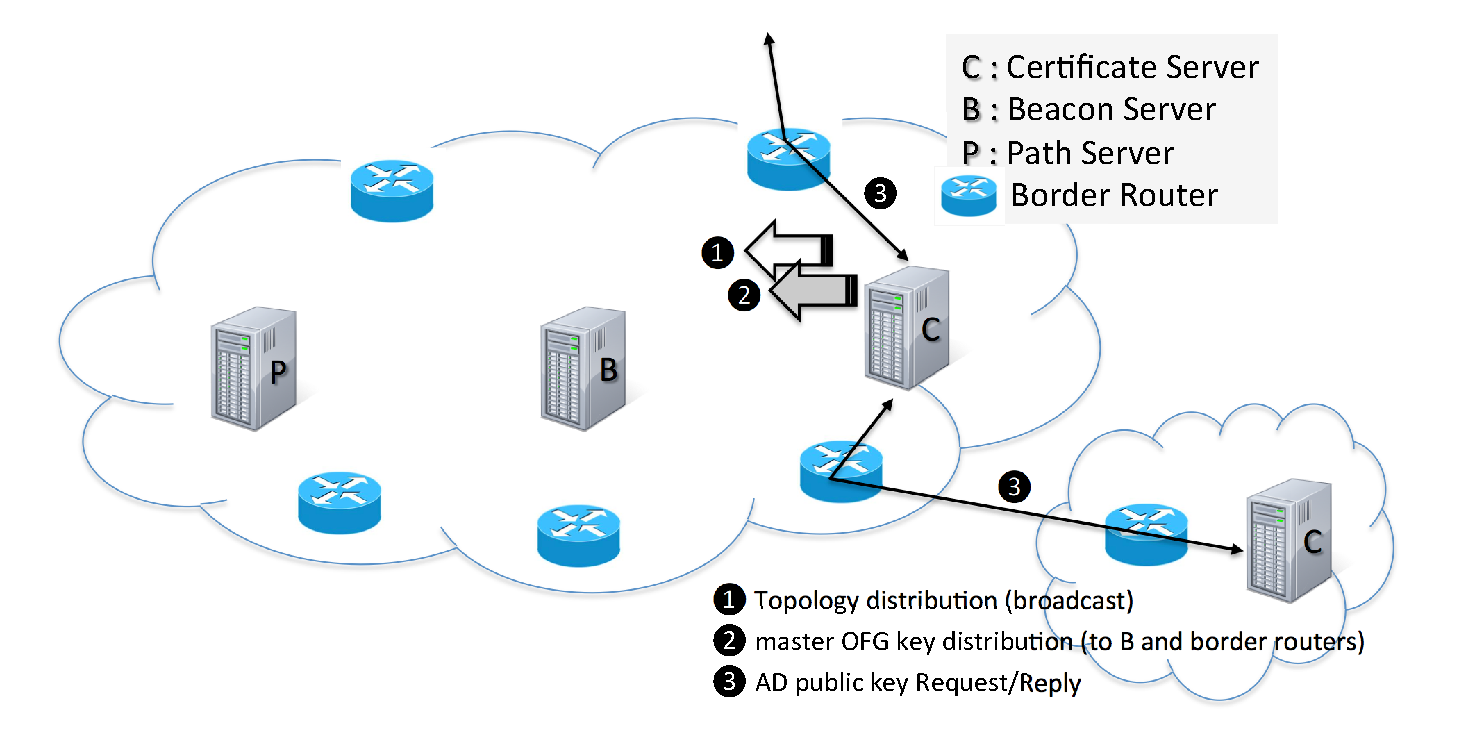
\includegraphics[width=.9\columnwidth]{./fig/cs_message.eps}
\caption{Certificate Server messages.}\label{fig:cs-message}
\end{figure*}

\noindent{\bf AD certificate: } The certificates of all participating \ADs to an \ISD are issued by the certificate authority of \ISD and stored at \ISDC \ADs and the owner of the certificates. Certificate servers are responsible for managing a certificate database and providing certificates to requesting \ADs. An \AD certificate contains the public key of an \AD signed by the \ISD's certificate authority. An \AD, using \AD certificates, verifies the signatures of other \ADs in inter-\AD communication (e.g., PCBs signed by its providers).

The {\em \ISDC certificate server} holds all certificates of \ADs that belong to the \ISD and provides them to requesting \ADs. Only certificate servers are allowed to request \AD certificates and for the request, they need to provide their signature for the request. A certificate request cannot be directly made to \ISDC certificate server, yet should traverse all \CSs on the path to \ISDC. For example, when a \STUB \AD requests an \AD's certificate (to \ISDC), this request is forwarded to the \CS of its provider \AD. Border routers can forward the request to the \CS (by putting the server address to the destination AID field) since they keep track of the server locations; viz., topology distribution below. The provider's \CS immediately responds to the request if the requested certificate is present in its local cache (or database) or (2) requests the certificate to its provider \AD. This procedure continues recursively up to \ISDC, until the certificate is found and returned to the requester. The \CSs on the return path store the certificate so that they respond to any later request for  the same certificate immediately. 
\tenma{This part is similar to how DNS query works. For Certificate request message, should the Endpoint AD puts its signature for identity
verification? even if it just requests the ``public'' informaiton, i.e., certificate.}

\noindent{\bf Entity certificate: } An \AD's \CS holds the certificates of all local entities such as routers, switches, servers, and gateways to secure intra-\AD communication. When an entity is added to an \AD, the entity is issued an certificate from the local certificate authority and register the certificate to the \CS. All border routers are configured to keep the \CS certificate of its own \AD to authenticate the messages from the \CS. Note that the border routers keep updated with the Opaque Field Generation (OFG) key and server list (in the topology file) by the \CS.


\section{Key Management}
A \CS shares a (master) secret key with each entity (server, router, or gateway) in the \AD, with which the \CS establishes a secure channel with those entities. The master secret key is pre-installed at individual entities when they join the \AD\tenma{Why we just use pre-installed certificate instead of using master secret key. Using symmetric cryptographic based on master secret may cause some problems}. The \CS generates a OFG key periodically (e.g., once a day) and distributes it to the \BS and border routers\tenma{securely? using authenticated-encryption based on the master secret key or envelope secure message based on asymmetric cryptography?}. Using this OFG key, the \BS creates PCBs (more specifically, opaque fields in PCBs) and the border routers verify the opaque fields. 

\begin{itemize}
\item {Offline Key: } master secret key
\item {Online Key: } OFG key
\end{itemize}



\section{Topology}
A \CS maintains the \AD topology file that describes the list of entities and their configuration information.
All entities are assigned a unique AID and type. The entity types currently defined in SCION and the information that need to be specified by each type are as follows.
AID is the authenticated ID of an entity and is used for an address identifier \chris{AID is also the abbreviation for AD ID and is used in \RT file, this is a bit confusing}; and the type identifier is specified in the parenthesis.

\begin{itemize}
\item Certificate Server (TYPE\_CS): AID \tenma{AID are same for different entities, such as Cert, Beacon, Path Servers? Here they look the same. My suggestion is using some real instances to describe it in Figure~4.}
\item Beacon Server (TYPE\_BS): AID
\item Path Server (TYPE\_PS): AID
\item Border Router (TYPE\_BR): AID, interface ID, neighbor \AD (AD ID), \AD relationship (P,C,E)\newline
	* P:Provider, C:Customer, E:pEer
\item Gateway (TYPE\_GW): AID, protocol 
\end{itemize}
Each interface card in a border router is assigned a unique interface ID among all interfaces within an AD to expedite packet forwarding. That is, an ingress router, on receiving a packet, forwards the packet directly to the egress router and the egress router sends out the packet to the interface ID specified in the packet. The information regarding the interface ID to neighbor \AD mapping and \AD relationship is used by the \BS when the \BS makes a PCB propagation decision (e.g., which PCB to propagate to which \AD). Furthermore, neighbor \AD can be used for internal traffic engineering (e.g., \AD-level bandwidth allocation and enforcement). A gateway is used to connect a SCION network to a heterogeneous network that runs with a different protocol (e.g., IPv4, IPv6). 
The \AD topology is stored in XML format as shown in Figure~\ref{fig:topology-file}.

%\begin{figure}[h]
%\centering
%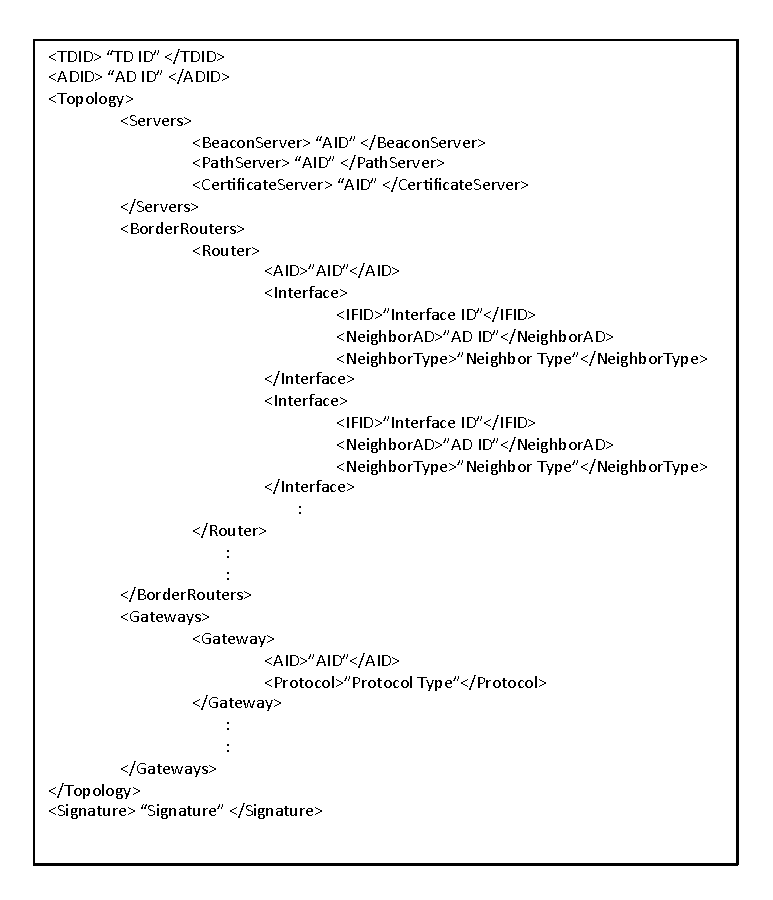
\includegraphics[width=.7\columnwidth]{./fig/topologyfile.eps}
%\caption{Topology File Format}\label{fig:topology-file}
%\end{figure}

\begin{SaveVerbatim}{TopSection}
<Topology ISDID="ISD ID" ADID="AD ID">	
<!-- put ISDID and ADID here beacuse a valid xml only has one root element -->
	<Servers>
		<BeaconServer>"AID"</BeaconServer>
		<PathServer>"AID"</PathServer>
		<CertificateServer>"AID"</CertificateServer>
	</Servers>
	<BorderRouters>
		<Router>	
		<!-- Why we just switch single field to property header -->
			<AID>"AID"</AID>
			<Interface>
				<IFID></IFID>
				<NeighborAD>"AD ID"</NeighborAD>
				<NeighborType>"AD ID"</NeighborType>
			</Interface>
			<Interface>
				<IFID></IFID>
				<NeighborAD>"AD ID"</NeighborAD>
				<NeighborType>"AD ID"</NeighborType>
			</Interface>
				...
		</Router>
		<Router>
			...
		</Router>
			....
	</BorderRouters>
	<Gateways>
		<Gateway>
			<AID>"AID"<AID>
			<Protocol>"Protocol Type"</Protocol>
		</Gateway>
			...
	</Gateways>
	<Signature>"Signature"<Signature>
</Topology>
\end{SaveVerbatim}

\begin{figure}[h]
\centering
%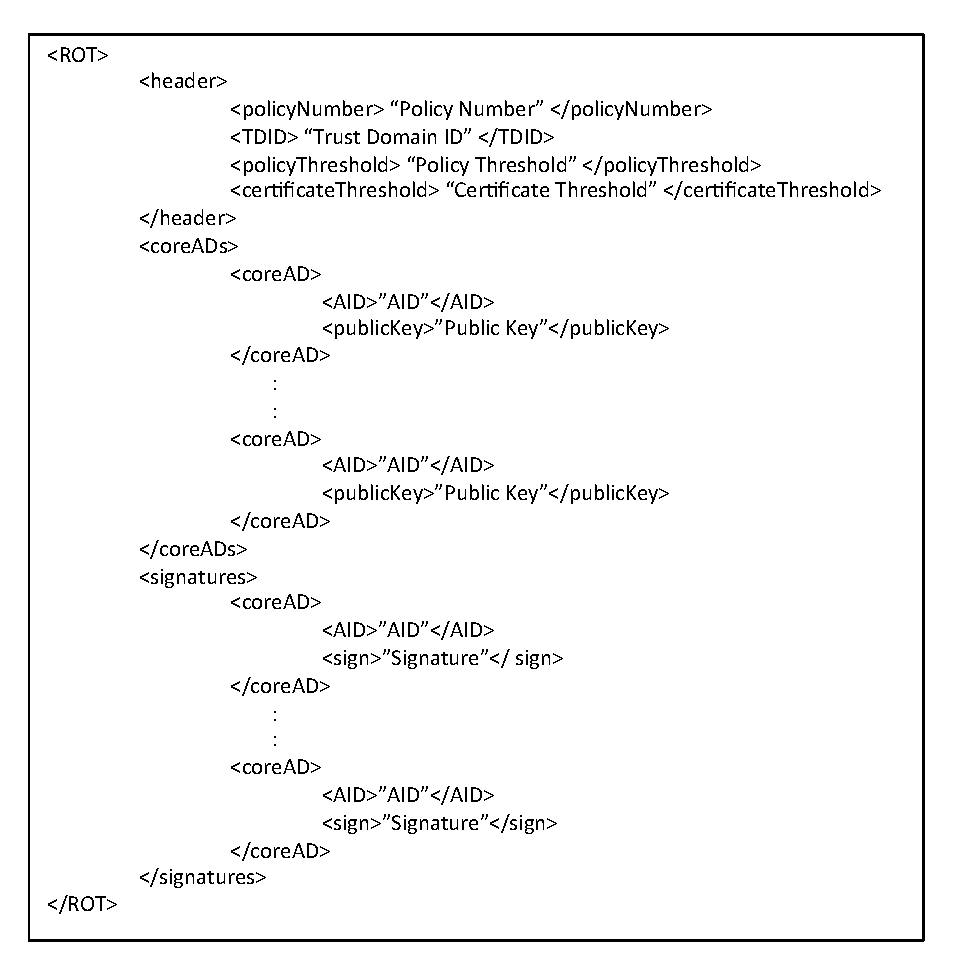
\includegraphics[width=.7\columnwidth]{./fig/rotfile.eps}
%\caption{\RT File Format}\label{fig:rot-file}
\begin{center}
	\fbox{
		\begin{minipage}{\columnwidth}
			\BUseVerbatim[fontsize=\footnotesize]{TopSection}
		\end{minipage}
	}
\end{center}
\caption{Topology File Format}\label{fig:topology-file}
\end{figure}


The \CS distributes server AIDs to border routers so that the border routers forward packets to necessary services. The border routers forward
\begin{itemize}
\item Certificate Request/Response to the \CS
\item PCB to the \BS
\item Path Registration/Resolution to the \PS(s)
\end{itemize}

To forward special packets (i.e., non-data packets listed above) to correct servers, the border routers write the packet's destination AID with the corresponding server's AID. Once the servers process the packets, they remove the destination AID field. This not only make the packet forwarding transparent outside the \AD but also would prevent targeted attacks against those servers.

\section{Bootstrapping}
\noindent {\bf \ISDC \CS: }
The \ISDC is the \RT of an \ISD and the \ISDC \CS has the essential information for establishing \RT. Hence, the \ISDC \CS must be able to start independently. The \ISDC \CS has a local copy of \RT file and all \AD certificates that it has issued (or under itself in \ISDC hierarchy) in its database. The \ISDC \CS communicates with other \ISDC \CSs (if any) in the same \ISD to update the most recent \RT file and necessary (missing) certificates.

\noindent {\bf \AD \CS: } The \CS is the \RT of an \AD as well. The \CS stores the certificates of local entities and the topology file. On its startup, the \CS broadcast server locations inside the \AD and the current OFG key to all border routers. The \CS essentially needs to store the most recent OFG key so that the \CS would not invalidate all opaque fields that are currently being used due to its instantaneous failure. Furthermore, the \CS stores the most recently used (expired) OFG key to help recover the \BS and border routers from their failure. Since an opaque field is valid for 1 day, a border router's Key Table should keep two OFG keys (i.e., the current and previous OFG keys).

\noindent{\bf Assumptions: }
For bootstrapping {em trust}, we make the following assumptions.
\begin{itemize}
\item Trust the \CS(s) in keeping the latest \RT file \chris{How is the \RT kept up to date? Analyzing the communication between BS and CS is needed}
\item \ADs know some public keys of \ISDC \ADs \soobum{necessary? This seems to be a vague assumption} \tenma{Should be. I think it
might be the initial trust. some could changed to ``threshold number''?}
\item \ADs can access the \CS \soobum{This is not an assumption, but a necessary condition for the very initial bootstrapping of SCION}
\end{itemize}
